\subsection{IFIT3} \label{IFIT3}
\subsubsection{Nascent Human and Monkey IFIT3 in a Simplified System of pseudo-IBs} \label{Nascent Human and Monkey IFIT3 in a Simplified System of pseudo-IBs}
\myparagraph{vero hnhp}
Detecting magenta: endogenous monkey IFIT3 \newline
Detecting cyan: human pIB \newline
Cell Line: VERO \newline
Treatment: hNhP \newline

Nascent monkey IFIT3 seems to behave a if he pIB was not here. This means I has diffused phenotype. One exception is the top panel (shown with the arrow) which hints at concentrated IFIT3 at the edge of the pIBs. We do not know the localisation with respect to the pIB filaments as none were found in the slides. This data is as well supported by z stack measurements.

\begin{figure}
    \centering
    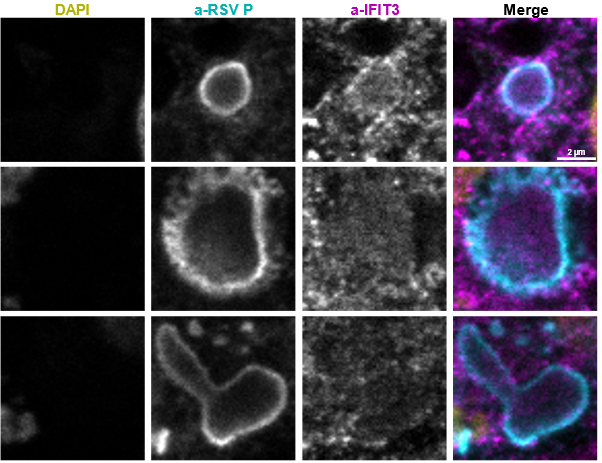
\includegraphics[width=1\linewidth]{08. Chapter 3/Figs/04. IFIT3/01. vero hnhp.png}
    \caption[i3 vero hnhp]{i3 vero hnhp}
    \label{i3 vero hnhp}
\end{figure}

\subsubsection{Nascent Human and Bovine IFIT3 Localisation During h/bRSV Infection} \label{Nascent Human and Bovine IFIT3 Localisation During h/bRSV Infection}
\myparagraph{hIFIT3 Localisation During hRSV Infection} \label{hIFIT3 Localisation During hRSV Infection}
\mysubparagraph{a549 hrsv}
Detecting magenta: endogenous human IFIT3 \newline
Detecting cyan: human IB \newline
Cell Line: A549 \newline
Treatment: hRSV \newline

Nascent human IFIT3 seems to have mainly diffused phenotype (top and bottom panel) with occasional exclusion without any marked IFIT3 concentration adjacent to the IB structure (middle panel).

\begin{figure}
    \centering
    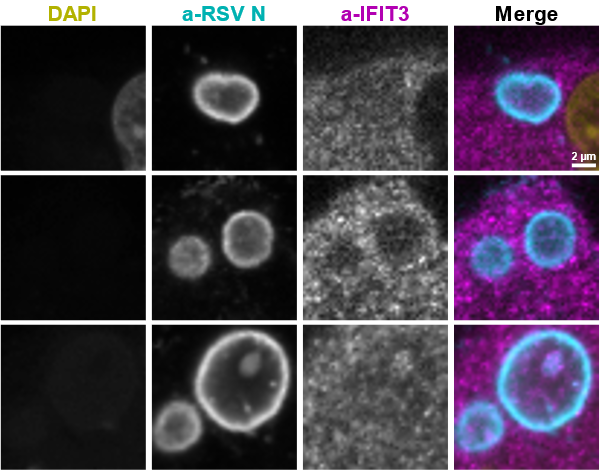
\includegraphics[width=1\linewidth]{08. Chapter 3/Figs/04. IFIT3/02. a549 hrsv.png}
    \caption[i3 a549 hrsv]{i3 a549 hrsv}
    \label{i3 a549 hrsv}
\end{figure}

\mysubparagraph{beas2b hrsv}
Detecting magenta: endogenous human IFIT3 \newline
Detecting cyan: human IB \newline
Cell Line: BEAS2B \newline
Treatment: hRSV \newline

\begin{figure}
    \centering
    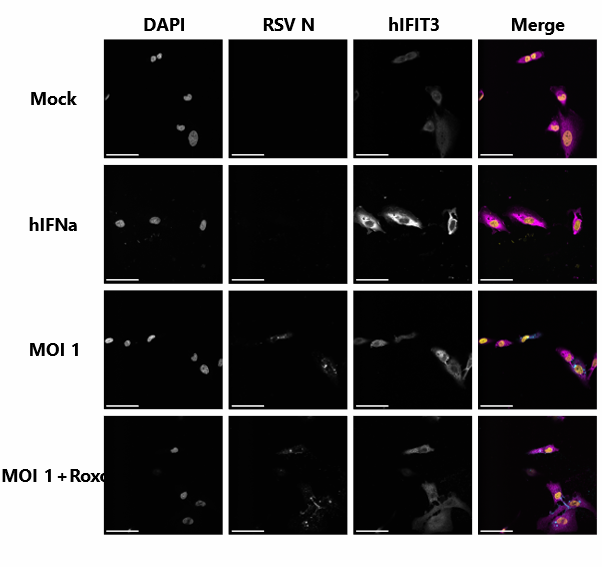
\includegraphics[width=1\linewidth]{08. Chapter 3/Figs/04. IFIT3/03. beas2b hrsv.png}
    \caption[i3 beas2b hrsv]{i3 beas2b hrsv}
    \label{i3 beas2b hrsv}
\end{figure}

\myparagraph{bIFIT3 Localisation During h/bRSV Infection} \label{bIFIT3 Localisation During h/bRSV Infection}
\mysubparagraph{mdbk hrsv}
some text

\begin{figure}
    \centering
    
\includegraphics[width=0.5\linewidth]{06. Chapter 1//Figs/00. placeholder.png}
    \caption[i3 mdbk hrsv]{i3 mdbk hrsv}
    \label{i3 mdbk hrsv}
\end{figure}

\mysubparagraph{mdbk brsv}
Detecting magenta: endogenous bovine IFIT3 \newline
Detecting cyan: bovine IB \newline
Cell Line: MDBK \newline
Treatment: bRSV dSH + bIFNa \newline

In this experiment the nascent bovine IFIT3 was consistently concentrated inside IBs. In some IBs the IFIT3 signal showed signs of sub-concentrations within the inclusions (bottom panel; highlighted with arrows), resembling IBAGs (inclusion body associated granules).

Subsequent experiments did not recapitulate the IFIT3 inclusions. It however shows signal which is almost identical to what is observed with IFIT5 in MDBKs during bRSV infection i.e., decrease, but not complete abolishment of IFIT3 signal inside the IB structure (top panel), and IB boundary exclusion while maintaining similar levels of signal intensity between cytoplasmic and intra IB stain.

\begin{figure}
    \centering
    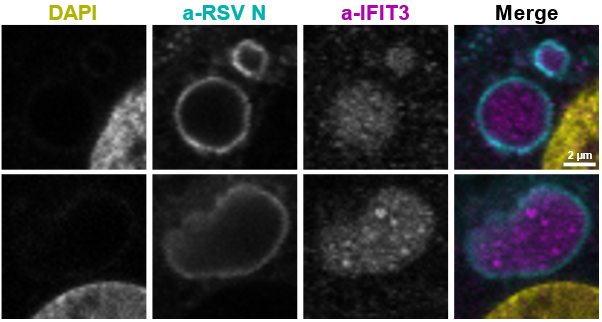
\includegraphics[width=1\linewidth]{08. Chapter 3/Figs/04. IFIT3/04. mdbk brsv.png}
    \caption[i3 mdbk brsv]{i3 mdbk brsv}
    \label{i3 mdbk brsv}
\end{figure}


\subsubsection{Exogenously Expressed hIFIT3-FLAG During RSV Infection} \label{Exogenously Expressed hIFIT3-FLAG During RSV Infection}
\myparagraph{bi3 + hrsv brsv}
Cell Line: VERO \newline
Treatment: hRSV-GFP \newline
Detecting magenta: exogenous bovine IFIT3 \newline
Detecting cyan: human IB \newline

Overexpressed bIFIT3-FLAG was observed to colocalise with hRSV inclusion bodies (top panel; highlighted with arrows), as well as being excluded from the hRSV IBs, without any signs of IFIT3 signal on the periphery of the IB structures (middle and bottom panel). This data is supported by z stack measurements.

\begin{figure}
    \centering
    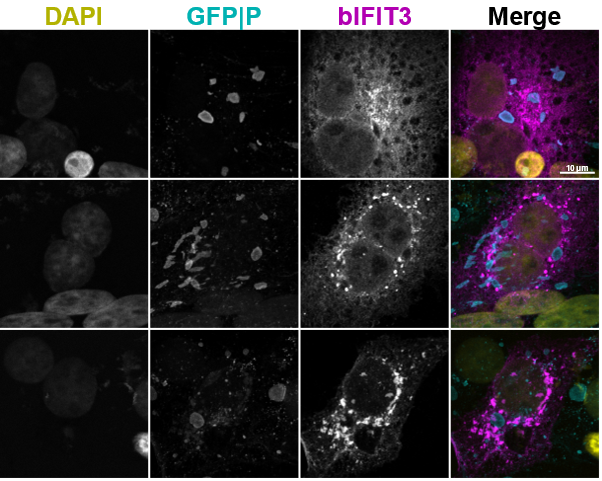
\includegraphics[width=1\linewidth]{08. Chapter 3/Figs/04. IFIT3/05. bi3 hrsv.png}
    \caption[bi3 + hrsv]{bi3 + hrsv}
    \label{bi3 + hrsv}
\end{figure}

Cell Line: VERO \newline
Treatment: bRSV-GFP \newline
Detecting magenta: exogenous bovine IFIT3 \newline
Detecting cyan: bovine IB \newline

Very similar phenotype is observed for overexpressed bIFIT3-FLAG in bRSV infected cells. We see colocalization with IB (top panel) as well as exclusion from the structure without any signs of IFIT3 signal on the periphery of the IB structure (bottom panel). This data is as well supported by z stack measurements.

\begin{figure}
    \centering
    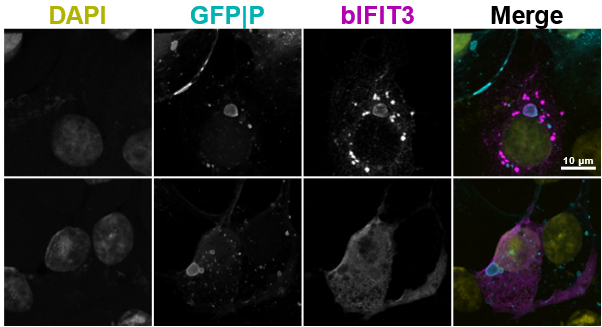
\includegraphics[width=1\linewidth]{08. Chapter 3/Figs/04. IFIT3/06. bi3 brsv.png}
    \caption[bi3 + brsv]{bi3 + brsv}
    \label{bi3 + brsv}
\end{figure}

\subsubsection{Summary} \label{Summary-i3}
Endogenous monkey IFIT3 seems to be diffuse through the human pIB structures (with maybe a small hint of colocalization). Nascent human IFIT3 during hRSV infection is either excluded from IB structure or is diffused through the structure. Occasionally it colocalises to the IB ring. Nascent bIFIT3 during bRSV infection either siphons inside IBs and shows sub-IB granules or is excluded from the IB boundary with slightly decreased signal inside of the IB. Overexpressed bIFIT3 behaves equally between hRSV and bRSV infection, that is it sometimes colocalises with the IB structure and sometimes is completely excluded from the structure.